\documentclass[sigconf]{acmart}
\settopmatter{printacmref=false, printccs=false, printfolios=true}
\renewcommand\footnotetextcopyrightpermission[1]{}
\acmConference[ComPar 26/27]{ComPar 26/27 Project Assignment 1}{November 2026}{}

\usepackage{booktabs}
\usepackage{graphicx}
\sloppy  % long \texttt identifiers otherwise overflow the narrow columns

\begin{document}
\title{Performance Engineering of a Spark Pipeline over NYC Taxi Trips}

\author{Gonçalo Costa (64548)}
\email{gfe.costa@campus.fct.unl.pt}

\begin{abstract}
This report describes how I profiled and optimised a PySpark pipeline over the
NYC Yellow Taxi trip data. I started with a simple version and used the Spark
UI metrics and the execution plans to find the slow parts: the raw data was
read many times, one window function shuffled the whole table and spilled to
disk, and some aggregations were repeated. After six changes, executor CPU
went down 46\% and shuffled data 93\% on my machine, and run time went down
31\% on a 3-worker Docker cluster. Adding workers in Docker did not make the
pipeline faster, and I explain why.
\end{abstract}

\keywords{Apache Spark, performance engineering, profiling, shuffle, caching}

\maketitle

%---------------------------------------------------------------------------
\section{Introduction}

I used the NYC Taxi \& Limousine Commission Yellow Taxi trip
records~\cite{tlc}. There is one Parquet file per month; for 2024 this is
41.2\,M records and 616\,MB. There is also a small zone table with 265 rows.
The pipeline runs the three mandatory operations (M1 cleaning, M2 temporal
demand, M3 zone statistics) and two optional ones: O1 fare anomalies and O2
origin--destination flows.

This workload is interesting for performance because all operations read the
same big table but group it by different keys, so a simple version does one
scan and one shuffle per operation. The zone table is very small, so the join
strategy matters. Also, a few zones (airports, Midtown) have most of the
trips, which causes skew when data is partitioned by zone.

I chose \textbf{O1} because the natural way to write it is a window function,
which shuffles every trip and suffers from the zone skew. I chose \textbf{O2}
because it has a large aggregation (routes $\times$ months), joins the zone
table twice, and builds three outputs from the same intermediate result, so it
is easy to recompute things by accident.

%---------------------------------------------------------------------------
\section{Pipeline}

The pipeline (\texttt{src/main.py}) uses Spark~\cite{zaharia2012rdd} with the
DataFrame API~\cite{armbrust2015sparksql}. Each operation is a function that
takes the clean trips and returns a result. I used the DataFrame API instead
of SQL strings because it is easier to compose and check, and the plans are
the same. Each optimisation can be turned on or off with the \texttt{--opt}
flag, so the baseline and the optimised version run from the same code.

\textbf{M1.} The monthly files do not all use the same types (for example
\texttt{passenger\_count} is sometimes \texttt{int64} and sometimes
\texttt{double}), so I read each file, cast it to a fixed schema, and join
them with a union. Each cleaning rule sets one bit in a mask column; the
statistics per year are one aggregation over the mask, and the clean data is
where the mask is 0. I added one extra rule: pickups outside the month of the
file (420 records in 2024).

\textbf{M2} adds the pickup borough and aggregates by (borough, weekday,
hour), written partitioned by borough. \textbf{M3} aggregates by (zone, month)
and uses windows for the rank in each borough, the 3-month rolling share, and
the 1.5$\sigma$ flag against the previous three months. \textbf{O1} computes
the mean and $\sigma$ of fare per km for each (zone, hour), flags trips above
mean$+3\sigma$, and compares anomaly rates by borough, payment type and
weekday/weekend. \textbf{O2} counts trips per route and month, computes each
route's share of its zone's trips, the top-20 routes per borough, and the
routes whose share goes up in Q1 and down in Q3 (or the opposite).

\begin{figure}[t]
\scriptsize
\begin{verbatim}
 baseline (window)                   o1_agg
 HashAggregate(borough,pay,day)      HashAggregate(borough,pay,day)
 +- Exchange                         +- Exchange
    +- BroadcastHashJoin(zones)         +- BroadcastHashJoin(zones)
       +- Window avg,stddev                +- BroadcastHashJoin(PU,hour)
          +- Sort(PU,hour)                    :  +- BroadcastExchange
             +- Exchange(PU,hour,200)         :     +- HashAggregate
                +- FileScan (all trips)       :        +- Exchange
                                              :           +- partial agg
                                              :              +- FileScan
                                              +- FileScan (all trips)
\end{verbatim}
\caption{O1 physical plan, simplified. Left: the window shuffles and sorts all
trips. Right: only small partial aggregates are shuffled, and the 6\,k bucket
statistics are broadcast back.}
\label{fig:plan}
\end{figure}

%---------------------------------------------------------------------------
\section{Profiling and Baseline}

\textbf{Setup.} Local: Apple M1 (8 cores), 8\,GB RAM, Java 21, Spark 4.0.1 in
\texttt{local[*]} mode with a 3\,GB driver. Docker: Spark standalone cluster
(\texttt{apache/spark:4.0.1-python3}) on the same laptop, with one master
(also running the 1\,GB driver) and 1 to 3 workers with 2 cores and a 640\,MB
executor each. Docker only has 4\,GB of memory, so 3 workers was the maximum.
Data: 2024, 12 files, 41.2\,M records. AQE is on (default).

\textbf{Measuring.} Each operation runs in its own Spark job group. At the end
of a run, a small profiler reads the Spark UI REST API and saves, for every
stage, the number of tasks, input, shuffle, spill, CPU and GC time, and task
time quantiles. I also saved the plans with \texttt{explain(mode="extended")}.

\textbf{Problems with the first measurements.} My first numbers were not
reliable. The project folder was synced with iCloud, so every output was
uploaded and the sync processes pushed the load above 40. I moved data and
outputs out of that folder. With a 4\,GB driver the laptop was swapping, and
the same run took between 86 and 120\,s, so I lowered it to 3\,GB. Even after
this, wall-clock time on the laptop still varied up to $2\times$. For local
results I therefore use shuffle bytes, input bytes, tasks and executor CPU
time, which change much less. Each configuration ran 3 times, mixed with the
others, and I report the median.

\textbf{Baseline} (local, median of 3): 144\,s, 617\,s of executor CPU, 851
tasks, 4.1\,GB read, 547\,MB shuffled and 234\,MB spilled. Per operation
(CPU s / input MB / shuffle MB): M1 42/515/0, M2 65/515/2, M3 133/1030/3,
O1 154/520/386, O2 212/1545/157.

\textbf{Bottlenecks.}
\emph{B1: the O1 window.} The plan (Fig.~\ref{fig:plan}) has an
\texttt{Exchange} on (zone, hour) followed by a \texttt{Sort} and a
\texttt{Window}. All 35\,M trips are shuffled (386\,MB) just to compute a mean
and a $\sigma$ per bucket. AQE merges this into 9 tasks of about 10\,s each,
and the stage spills 234\,MB to disk. It is the slowest stage.
\emph{B2: repeated work.} Nothing is reused, so the Parquet files are read 9
times (4.1\,GB): once per operation, twice for M3 and three times for O2. M3
also has a \texttt{SortMergeJoin} with its own borough totals.
\emph{B3: skew that is not real.} In the scan stages the slowest task takes
70--118$\times$ the median, which looks like skew. But the median task reads 0
records. Each file has only 3--4 row groups (44 in total) and Spark creates 96
tasks, so 52 tasks have nothing to read. The real limit is that a scan can use
at most 44 tasks.

%---------------------------------------------------------------------------
\section{Optimisation Study}

The changes were applied one after the other, starting with the biggest
bottleneck. For each one I checked that the results are the same as the
baseline (\texttt{scripts/compare\_outputs.py}).

\subsection{O1: aggregate and broadcast (\texttt{o1\_agg})}
\emph{Problem:} B1. \emph{Idea:} there are only $263\times24\approx6$\,k
buckets, so a \texttt{groupBy} shuffles very little and its result is small
enough to broadcast. \emph{Change:} \texttt{groupBy(zone, hour)} with
\texttt{avg} and \texttt{stddev}, then a broadcast join back to the trips.
\emph{Result:} O1 shuffle 386\,$\to$\,7.5\,MB, no more spill, O1 CPU
154\,$\to$\,134\,s. The gain is smaller than expected because the trips are
now read twice (once for the statistics, once for the join).

\subsection{O2: aggregate first, reuse the result (\texttt{o2\_agg})}
\emph{Problem:} B2. O2 reads the data three times and joins the zone names on
all 35\,M trips before aggregating. \emph{Idea:} count first, so the join is
on about 1\,M rows, and keep the result so the three outputs use it.
\emph{Change:} aggregate by ids, join names on the counts, \texttt{persist}
the shares. \emph{Result:} O2 input 1545\,$\to$\,526\,MB, shuffle
157\,$\to$\,64\,MB, CPU 201\,$\to$\,125\,s. The number of tasks went up
(945\,$\to$\,1519) because AQE does not merge the partitions of a persisted
DataFrame.

\subsection{M3: one window instead of a self-join (\texttt{m3\_window})}
\emph{Problem:} B2. M3 computes its monthly table twice and joins it with the
borough totals. \emph{Idea:} a range window over the month, partitioned by
borough, already gives the borough total for the last 3 months.
\emph{Change:} replace the aggregate and join with that window.
\emph{Result:} M3 input 1030\,$\to$\,515\,MB, CPU 144\,$\to$\,76\,s, and the
\texttt{SortMergeJoin} is gone.

\subsection{Cache the cleaned trips (\texttt{cache})}
\emph{Problem:} the files are still read five times. \emph{Idea:} read once
and keep the cleaned trips in memory. \emph{Change:} \texttt{persist}
(memory and disk) before M1. \emph{Result:} total CPU 461\,$\to$\,372\,s.
The other operations got much cheaper (O1 149\,$\to$\,52\,s), but M1 went
from 30 to 159\,s because building the cache is expensive.
Two things did not work as expected. When I first tried the cache
\emph{before} fixing O1, the pipeline got slower and then failed with
\texttt{SparkOutOfMemoryError}: the cache took the memory that the O1 window
needed to sort. That is why O1 was fixed first. I also thought a second pass
over the cache in M1 came from an \texttt{orderBy}, but removing it changed
nothing: in Spark 4 the cache is built in its own stage and then read.

\subsection{Cache without compression (\texttt{cache\_nocompress})}
\emph{Problem:} the plan shows \texttt{ColumnarToRow} before the cache, so the
data is converted to rows and compressed again into columns. Building the
cache costs 133\,s of CPU, against 30\,s for a normal scan. \emph{Idea:}
compression is the expensive part, and the uncompressed cache still fits in
memory. \emph{Change:} set
\texttt{spark.sql.inMemory\-ColumnarStorage\-.compressed} to \texttt{false}.
\emph{Result:} cache 826\,$\to$\,989\,MB (+20\%), building it 139\,$\to$\,84\,s
of CPU ($-40\%$), total CPU 396\,$\to$\,351\,s.

\subsection{O2 with integer keys (\texttt{o2\_ids})}
\emph{Problem:} two O2 aggregations still cost 28\,s of CPU each for about 1\,M
rows, because they group by zone and borough names (strings).
\emph{Idea:} group by the integer ids and add the names at the end.
\emph{Change:} \texttt{groupBy} on ids only, then a broadcast join with the
names. \emph{Result:} shuffle 75\,$\to$\,39\,MB, total CPU 351\,$\to$\,336\,s.

\begin{table}[t]
\caption{Optimisations applied one after the other, local, 2024. CPU is
executor CPU time (median of 3). The last three rows were measured in a second
session (cache: 372\,s first session, 396\,s second).}
\label{tab:opt}
\small
\begin{tabular}{lrrrr}
\toprule
configuration & CPU (s) & shuffle (MB) & spill (MB) & tasks \\
\midrule
baseline & 617 & 547 & 234 & 851 \\
+ o1\_agg & 585 & 169 & 0 & 945 \\
+ o2\_agg & 518 & 76 & 0 & 1519 \\
+ m3\_window & 461 & 75 & 0 & 1420 \\
+ cache & 372 / 396 & 75 & 0 & 1516 \\
+ cache\_nocompress & 351 & 75 & 0 & 1514 \\
+ o2\_ids & 336 & 39 & 0 & 1515 \\
\midrule
total change & $-46\%$ & $-93\%$ & $-100\%$ & $+78\%$ \\
\bottomrule
\end{tabular}
\end{table}

\subsection{How much does AQE help?}
All the runs above use Adaptive Query Execution, which is on by default and
re-plans each stage at runtime from the real shuffle sizes. To see its effect
I ran the optimised pipeline with \texttt{spark.sql.adaptive.enabled=false}
(2 runs each). Without AQE the pipeline runs 3384 tasks instead of 1515
($2.2\times$), because every shuffle keeps the default 200 partitions instead
of being merged, and executor CPU goes up 20\% (366\,$\to$\,440\,s, median).
O2 suffers most (CPU 106\,$\to$\,164\,s), since it has the most small
shuffles. Shuffle bytes barely change (39\,$\to$\,44\,MB) and there is no
spill in either case. The skew-join part of AQE does not apply here: after the
optimisations all joins are broadcast joins.

%---------------------------------------------------------------------------
\section{Analysis}
\label{sec:analysis}
In Docker I ran the optimised pipeline \emph{without} the cache. With 640\,MB
executors, building the cache failed with \texttt{OutOfMemoryError}, so the
cache only helps when executors have enough memory.

\textbf{Cluster baseline.} With 3 workers the baseline takes 411\,s and the
optimised version 284\,s ($-31\%$). Shuffle goes from 544 to 38\,MB, and the
biggest gains are in O2 (165\,$\to$\,68\,s) and M3 (73\,$\to$\,40\,s).

\begin{figure}[t]
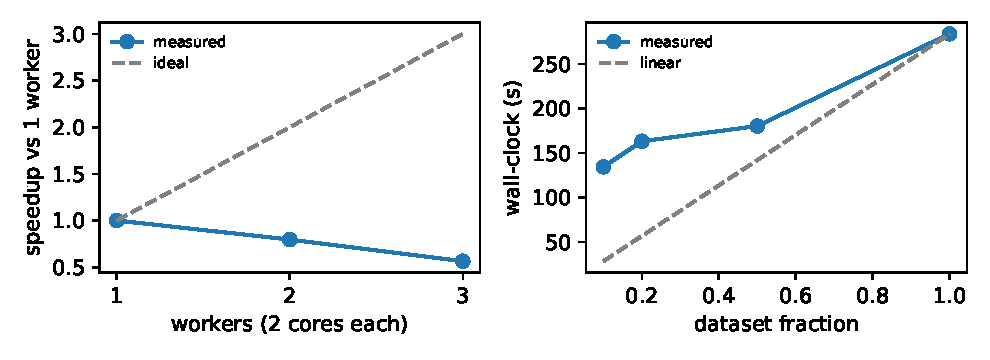
\includegraphics[width=\columnwidth]{figures/scaling.pdf}
\caption{Docker cluster, optimised pipeline. Left: speedup compared to 1
worker (2 cores each). Right: time vs.\ fraction of the data, 3 workers.}
\label{fig:scaling}
\end{figure}

\textbf{Cluster size} (Fig.~\ref{fig:scaling}, left). With 1, 2 and 3 workers
the pipeline takes 160, 201 and 284\,s, so the speedup is 0.80 and 0.56 and
the efficiency 0.40 and 0.19. More workers made it \emph{slower}. The work did
not change (same 514\,MB read, about the same shuffle), but the total executor
CPU went up with the number of cores (224, 554, 973\,s): each task needed more
CPU for the same data. I had two possible explanations: more JVMs and more
communication between them, or simply more cores competing on one laptop. To
check, I ran \emph{one} worker with 6 cores. It took 281\,s, the same as 3
workers with 2 cores, so the number of JVMs is not the cause. The ``cluster''
is one Docker VM on an M1, which has 4 fast and 4 slow cores, and the same VM
also runs the driver and serves the data files. With more than 2 busy cores,
tasks end up on the slow cores and wait for the VM. So this result comes from
the test setup, not from the pipeline; on a real cluster I would expect the
scans to scale, up to the limit of 44 row groups (B3).

\textbf{Dataset size} (Fig.~\ref{fig:scaling}, right). With 3 workers, 10, 20,
50 and 100\% of the data take 134, 163, 180 and 284\,s. So 10\% of the data
still takes 47\% of the time: scaling is clearly sub-linear. The reason is
that \texttt{--fraction} samples \emph{after} reading the files, so every run
still reads all 12 files (89\,s of scan stages at 10\%, 227\,s at 100\%).
Planning and scheduling are also a fixed cost. Only the work after the sample
gets smaller.

%---------------------------------------------------------------------------
\section{Discussion}

\textbf{What is still slow.} Building the cache is now the most expensive step
(84\,s of CPU, about a quarter of the total), because the rows are converted
and stored again. Writing the clean trips once to a new Parquet file could be
cheaper. The scans are limited to 44 tasks by the row groups; rewriting the
input with smaller row groups would allow more parallelism. Persisted
DataFrames keep 200 partitions, so many O2 stages run 200 very small tasks; a
\texttt{repartition} before \texttt{persist} would fix this. The zone skew is
still in the data, but after \texttt{o1\_agg} no stage partitions the raw trips
by zone, so it no longer hurts.

\textbf{Limitations.} Wall-clock time on my laptop is noisy, so the local
conclusions use CPU time and bytes, with only 3 runs each. The Docker cluster
runs on one machine, so it does not show network costs, and the DI cluster was
not used in this work. I only processed 2024; files before 2011 have no zone
ids and would be removed by M1.

\textbf{With more time} I would run on the DI cluster with more years, try the
fixes above, and run more repetitions of each test.

%---------------------------------------------------------------------------
\section*{Acknowledgements}
I used Claude (Anthropic) as an AI assistant for writing code, running tests,
making the charts and drafting the report.

\section*{Individual contributions}
Single-member project: Gonçalo Costa (64548), 100\%.

\bibliographystyle{acm}
\bibliography{refs}

\end{document}
